\documentclass[12pt,letterpaper]{article}
\usepackage{graphicx,textcomp}
\usepackage{natbib}
\usepackage{setspace}
\usepackage{fullpage}
\usepackage{color}
\usepackage[reqno]{amsmath}
\usepackage{amsthm}
\usepackage{fancyvrb}
\usepackage{amssymb,enumerate}
\usepackage[all]{xy}
\usepackage{endnotes}
\usepackage{lscape}
\newtheorem{com}{Comment}
\usepackage{float}
\usepackage{hyperref}
\newtheorem{lem} {Lemma}
\newtheorem{prop}{Proposition}
\newtheorem{thm}{Theorem}
\newtheorem{defn}{Definition}
\newtheorem{cor}{Corollary}
\newtheorem{obs}{Observation}
\usepackage[compact]{titlesec}
\usepackage{dcolumn}
\usepackage{tikz}
\usetikzlibrary{arrows}
\usepackage{multirow}
\usepackage{xcolor}
\newcolumntype{.}{D{.}{.}{-1}}
\newcolumntype{d}[1]{D{.}{.}{#1}}
\definecolor{light-gray}{gray}{0.65}
\usepackage{url}
\usepackage{listings}
\usepackage{color}

\definecolor{codegreen}{rgb}{0,0.6,0}
\definecolor{codegray}{rgb}{0.5,0.5,0.5}
\definecolor{codepurple}{rgb}{0.58,0,0.82}
\definecolor{backcolour}{rgb}{0.95,0.95,0.92}

\lstdefinestyle{mystyle}{
	backgroundcolor=\color{backcolour},   
	commentstyle=\color{codegreen},
	keywordstyle=\color{magenta},
	numberstyle=\tiny\color{codegray},
	stringstyle=\color{codepurple},
	basicstyle=\footnotesize,
	breakatwhitespace=false,         
	breaklines=true,                 
	captionpos=b,                    
	keepspaces=true,                 
	numbers=left,                    
	numbersep=5pt,                  
	showspaces=false,                
	showstringspaces=false,
	showtabs=false,                  
	tabsize=2
}
\lstset{style=mystyle}
\newcommand{\Sref}[1]{Section~\ref{#1}}
\newtheorem{hyp}{Hypothesis}

\title{Problem Set 3}
\date{Due: November 19, 2022}
\author{Applied Stats/Quant Methods 1}


\begin{document}
	\maketitle
	\section*{Instructions}
	\begin{itemize}
		\item Please show your work! You may lose points by simply writing in the answer. If the problem requires you to execute commands in \texttt{R}, please include the code you used to get your answers. Please also include the \texttt{.R} file that contains your code. If you are not sure if work needs to be shown for a particular problem, please ask.
	\item Your homework should be submitted electronically on GitHub.
	\item This problem set is due before 23:59 on Sunday November 19, 2023. No late assignments will be accepted.

	\end{itemize}

		\vspace{.25cm}
	
\noindent In this problem set, you will run several regressions and create an add variable plot (see the lecture slides) in \texttt{R} using the \texttt{incumbents\_subset.csv} dataset. Include all of your code.

	\vspace{.5cm}
\section*{Question 1}
\vspace{.25cm}
\noindent We are interested in knowing how the difference in campaign spending between incumbent and challenger affects the incumbent's vote share. 
	\begin{enumerate}
		\item Run a regression where the outcome variable is \texttt{voteshare} and the explanatory variable is \texttt{difflog}.	
		
		\noindent Input :
			\lstinputlisting[language=R, firstline=42, lastline=48]{PS3.R}  
		
		
		Output:
			\begin{verbatim}
				
				> inc.sub$voteshare[is.na(inc.sub$voteshare)]
				numeric(0)
				> inc.sub$difflog[is.na(inc.sub$difflog)]
				numeric(0)
				
				Call:
				lm(formula = voteshare ~ difflog, data = inc.sub)
				
				Residuals:    
				 Min       1Q       Median     3Q        Max 
				 -0.26832 -0.05345 -0.00377  0.04780  0.32749
				 
				 Coefficients:            
				           Estimate  Std. Error   t value   Pr(>|t|)    
				 (Intercept) 0.579031   0.002251  257.19   <2e-16 ***
				 difflog     0.041666   0.000968   43.04   <2e-16 ***
				 --Signif. codes:  0 ‘***’ 0.001 ‘**’ 0.01 ‘*’ 0.05 ‘.’ 0.1 ‘ ’ 1
				 
				 Residual standard error: 0.07867 on 3191 degrees of freedom
				 Multiple R-squared:  0.3673,	Adjusted R-squared:  0.3671  
				 F-statistic: 1853 on 1 and 3191 DF,  p-value: < 2.2e-16
				
				\end{verbatim}
			\normalsize
			
			\begin{table}[!htbp] \centering   \caption{}   \label{} \begin{tabular}{@{\extracolsep{5pt}}lc} \\[-1.8ex]\hline \hline \\[-1.8ex]  & \multicolumn{1}{c}{\textit{Dependent variable:}} \\ \cline{2-2} \\[-1.8ex] & voteshare \\ \hline \\[-1.8ex]  difflog & 0.042$^{***}$ \\   & (0.001) \\   & \\  Constant & 0.579$^{***}$ \\   & (0.002) \\   & \\ \hline \\[-1.8ex] Observations & 3,193 \\ R$^{2}$ & 0.367 \\ Adjusted R$^{2}$ & 0.367 \\ Residual Std. Error & 0.079 (df = 3191) \\ F Statistic & 1,852.791$^{***}$ (df = 1; 3191) \\ \hline \hline \\[-1.8ex] \textit{Note:}  & \multicolumn{1}{r}{$^{*}$p$<$0.1; $^{**}$p$<$0.05; $^{***}$p$<$0.01} \\ \end{tabular} \end{table} 
		
		\vspace{10cm}
		
		\item Make a scatterplot of the two variables and add the regression line. 	
		
	\begin{figure}[h!]\centering
		\caption{\footnotesize Boxplot of $Y$ by $Region$.}\vspace{-1cm}
		\label{fig:plot_3c}
		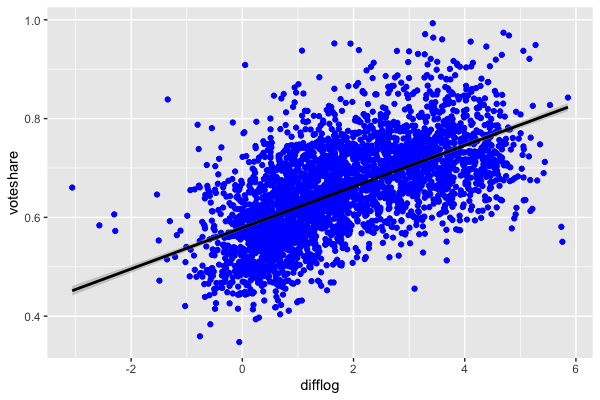
\includegraphics[width=.75\textwidth]{scatter1.png}
	\end{figure}
	
	\noindent From the scatterplot for model1, we can see that there is a positive correlation between the two variables. The slope in the output of the previous question is positive, and the p value is less than 0.001, which verifies this as well.
		\vspace{1cm}
		\item Save the residuals of the model in a separate object.
		
		\noindent Input coding:
		 	\noindent Input :
		 \lstinputlisting[language=R, firstline=107, lastline=108]{PS3.R}  
			\vspace{1cm}
			
			
		\item Write the prediction equation.
		
	\begin{equation}
		\hat{\text{{voteshare}}} = 0.579031 + 0.041666 \times \text{{difflog}}
	\end{equation}

	\noindent The prediction equation of model1  means when the difflog changes by one unit, the predicted voteshare changes by 0.041666 units. The multiple R-squared of this model is 0.3673, indicating that the model can explain approximately 36.7\% of the variance in voteshare. The explanatory varible  of difflog in the model is significant (p-value $<$ 0.05), indicating that difflog's prediction of voteshare is statistically significant.

	
\newpage

\section*{Question 2}
\noindent We are interested in knowing how the difference between incumbent and challenger's spending and the vote share of the presidential candidate of the incumbent's party are related.	\vspace{.25cm}
	\begin{enumerate}
		\item Run a regression where the outcome variable is \texttt{presvote} and the explanatory variable is \texttt{difflog}.
		
			\noindent Input :
		\lstinputlisting[language=R, firstline=51, lastline=53]{PS3.R}  
		
		
		Output:
		\begin{verbatim}
			
			> inc.sub$presvote[is.na(inc.sub$presvote)]
			numeric(0)
			
			Call:
			lm(formula = presvote ~ difflog, data = inc.sub)
			
			Residuals:    
			Min       1Q       Median     3Q        Max 
			-0.32196 -0.07407 -0.00102  0.07151  0.42743
			
			Coefficients:            
			Estimate  Std. Error   t value   Pr(>|t|)    
			(Intercept) 0.507583   0.003161  160.60   <2e-16***
			difflog     0.023837   0.001359   17.54   <2e-16 ***-
			--Signif. codes:  0 ‘***’ 0.001 ‘**’ 0.01 ‘*’ 0.05 ‘.’ 0.1 ‘ ’ 1
			
			Residual standard error: 0.1104 on 3191 degrees of freedom
			Multiple R-squared:  0.08795,	Adjusted R-squared:  0.08767 
			F-statistic: 307.7 on 1 and 3191 DF,  p-value: < 2.2e-16
			
		\end{verbatim}
		\normalsize
		
		\begin{table}[!htbp] \centering   \caption{}   \label{} \begin{tabular}{@{\extracolsep{5pt}}lc} \\[-1.8ex]\hline \hline \\[-1.8ex]  & \multicolumn{1}{c}{\textit{Dependent variable:}} \\ \cline{2-2} \\[-1.8ex] & presvote \\ \hline \\[-1.8ex]  difflog & 0.024$^{***}$ \\   & (0.001) \\   & \\  Constant & 0.508$^{***}$ \\   & (0.003) \\   & \\ \hline \\[-1.8ex] Observations & 3,193 \\ R$^{2}$ & 0.088 \\ Adjusted R$^{2}$ & 0.088 \\ Residual Std. Error & 0.110 (df = 3191) \\ F Statistic & 307.715$^{***}$ (df = 1; 3191) \\ \hline \hline \\[-1.8ex] \textit{Note:}  & \multicolumn{1}{r}{$^{*}$p$<$0.1; $^{**}$p$<$0.05; $^{***}$p$<$0.01} \\ \end{tabular} \end{table}
		
		
			\vspace{5cm}
		\item Make a scatterplot of the two variables and add the regression line. 
		
			\begin{figure}[h!]\centering
			\caption{\footnotesize Boxplot of $Y$ by $Region$.}\vspace{-1cm}
			\label{fig:plot_3c}
			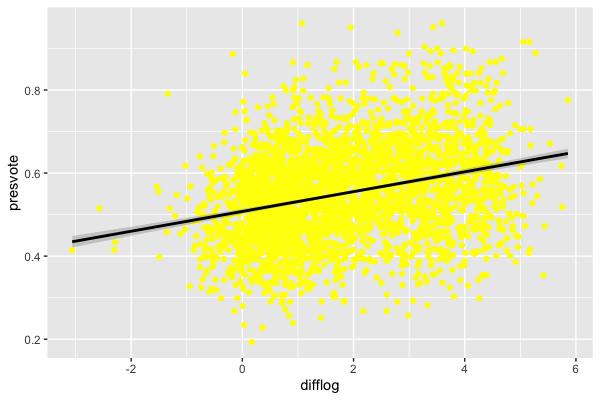
\includegraphics[width=.75\textwidth]{scatterplot2.png}
		\end{figure}
		
		\noindent From the scatterplot for model2, We can see that there is a positive correlation between the two variables. The slope in the output of the previous question is positive, and the p value is less than 0.001, which verifies this as well.
		
			\vspace{5cm}
		\item Save the residuals of the model in a separate object.	
		
			\noindent Input coding:
		\lstinputlisting[language=R, firstline=107, lastline=108]{PS3.R} 
		\vspace{1cm}
		
		\item Write the prediction equation.
		
		\begin{equation}
			\hat{\text{{presvote}}} = 0.507583 + 0.023837 \times \text{{difflog}}
		\end{equation}
		
		\noindent The prediction equation of model2  means when the difflog changes by one unit, the predicted presvote changes by 0.023837 units. The multiple R-squared of this model is 0.08795, indicating that the model can explain approximately 8.8\% of the variance in presvotes. However, according to the significance level of p-value, difflog in the model is significant (p-value $<$ 0.05), indicating that difflog's prediction of presvote is statistically significant.
	\end{enumerate}
	
	\newpage	
\section*{Question 3}

\noindent We are interested in knowing how the vote share of the presidential candidate of the incumbent's party is associated with the incumbent's electoral success.
	\vspace{.25cm}
	\begin{enumerate}
		\item Run a regression where the outcome variable is \texttt{voteshare} and the explanatory variable is \texttt{presvote}.
		
					\noindent Input :
		\lstinputlisting[language=R, firstline=56, lastline=57]{PS3.R}  
		
		
		Output:
		\begin{verbatim}
			
			Call:
			lm(formula = voteshare ~ presvote, data = inc.sub)
			
			Residuals:    
			Min       1Q       Median     3Q        Max 
			-0.27330 -0.05888  0.00394  0.06148  0.41365
			
			Coefficients:            
			Estimate  Std. Error   t value   Pr(>|t|)    
			(Intercept) 0.441330   0.007599   58.08   <2e-16 ***
			presvote     0.388018   0.013493   28.76   <2e-16 ***
			--Signif. codes:  0 ‘***’ 0.001 ‘**’ 0.01 ‘*’ 0.05 ‘.’ 0.1 ‘ ’ 1
			
			Residual standard error: 0.08815 on 3191 degrees of freedom
			Multiple R-squared:  0.2058,	Adjusted R-squared:  0.2056 
			F-statistic: 827 on 1 and 3191 DF,  p-value: < 2.2e-16
			
		\end{verbatim}
		\normalsize
		
		\begin{table}[!htbp] \centering   \caption{}   \label{} \begin{tabular}{@{\extracolsep{5pt}}lc} \\[-1.8ex]\hline \hline \\[-1.8ex]  & \multicolumn{1}{c}{\textit{Dependent variable:}} \\ \cline{2-2} \\[-1.8ex] & voteshare \\ \hline \\[-1.8ex]  presvote & 0.388$^{***}$ \\   & (0.013) \\   & \\  Constant & 0.441$^{***}$ \\   & (0.008) \\   & \\ \hline \\[-1.8ex] Observations & 3,193 \\ R$^{2}$ & 0.206 \\ Adjusted R$^{2}$ & 0.206 \\ Residual Std. Error & 0.088 (df = 3191) \\ F Statistic & 826.950$^{***}$ (df = 1; 3191) \\ \hline \hline \\[-1.8ex] \textit{Note:}  & \multicolumn{1}{r}{$^{*}$p$<$0.1; $^{**}$p$<$0.05; $^{***}$p$<$0.01} \\ \end{tabular} \end{table}
		
		
		\vspace{5cm}
		
		
			\vspace{5cm}
		\item Make a scatterplot of the two variables and add the regression line. 
		
			\begin{figure}[h!]\centering
			\caption{\footnotesize Boxplot of $Y$ by $Region$.}\vspace{-1cm}
			\label{fig:plot_3c}
			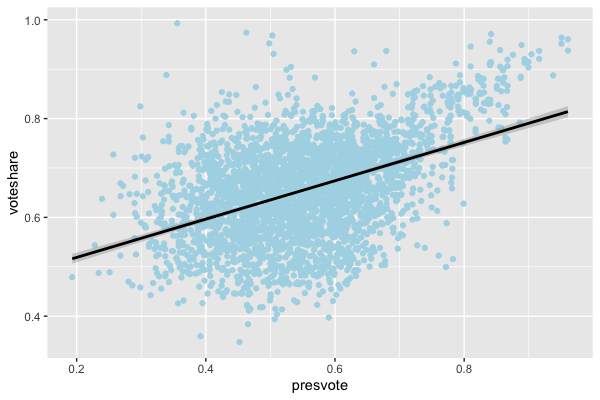
\includegraphics[width=.75\textwidth]{scatterplot3.png}
		\end{figure}
		
		\noindent From the scatterplot for model3, We can see that there is a positive correlation between the two variables. The slope in the output of the previous question is positive, and the p value is less than 0.001, which verifies this as well.
		
			\vspace{5cm}
		\item Write the prediction equation.
		
				\begin{equation}
			\hat{\text{{voteshare}}} = 0.441330  + 0.388018 \times \text{{presvote}}
		\end{equation}
		
		\noindent The prediction equation of model3 means when the presvote changes by one unit, the predicted voteshare changes by 0.388018 units. The multiple R-squared of this model is 0.2058, indicating that the model can explain approximately 20.6\% of the variance in voteshare. The  p-value of presvote in the model is significant (p-value $<$ 0.05), indicating that presvote's prediction of voteshare is statistically significant.
		\end{enumerate}
		
		
		
	\end{enumerate}
	

\newpage	
\section*{Question 4}
\noindent The residuals from part (a) tell us how much of the variation in \texttt{voteshare} is $not$ explained by the difference in spending between incumbent and challenger. The residuals in part (b) tell us how much of the variation in \texttt{presvote} is $not$ explained by the difference in spending between incumbent and challenger in the district.
	\begin{enumerate}
		\item Run a regression where the outcome variable is the residuals from Question 1 and the explanatory variable is the residuals from Question 2.	
				
		\noindent Input :
		\lstinputlisting[language=R, firstline=59, lastline=60]{PS3.R}  
		
		
		Output:
		\begin{verbatim}
			Call:
			lm(formula = residual1 ~ residual2)
			
			Residuals:    
			 Min       1Q       Median     3Q        Max 
			-0.25928 -0.04737 -0.00121  0.04618  0.33126 
			
			Coefficients:            
			Estimate  Std. Error   t value   Pr(>|t|)    
			(Intercept) -1.942e-18  1.299e-03    0.00        1 
			residual2     2.569e-01  1.176e-02   21.84   <2e-16 ***
			--Signif. codes:  0 ‘***’ 0.001 ‘**’ 0.01 ‘*’ 0.05 ‘.’ 0.1 ‘ ’ 1
			
			Residual standard error:  0.07338 on 3191 degrees of freedom
			Multiple R-squared:  0.13,	Adjusted R-squared:      0.1298 
			F-statistic: 477 on 1 and 3191 DF,  p-value: < 2.2e-16
			
		\end{verbatim}
		\normalsize
		
		\begin{table}[!htbp] \centering   \caption{}   \label{} \begin{tabular}{@{\extracolsep{5pt}}lc} \\[-1.8ex]\hline \hline \\[-1.8ex]  & \multicolumn{1}{c}{\textit{Dependent variable:}} \\ \cline{2-2} \\[-1.8ex] & residual1 \\ \hline \\[-1.8ex]  residual2 & 0.257$^{***}$ \\   & (0.012) \\   & \\  Constant & $-$0.000 \\   & (0.001) \\   & \\ \hline \\[-1.8ex] Observations & 3,193 \\ R$^{2}$ & 0.130 \\ Adjusted R$^{2}$ & 0.130 \\ Residual Std. Error & 0.073 (df = 3191) \\ F Statistic & 476.975$^{***}$ (df = 1; 3191) \\ \hline \hline \\[-1.8ex] \textit{Note:}  & \multicolumn{1}{r}{$^{*}$p$<$0.1; $^{**}$p$<$0.05; $^{***}$p$<$0.01} \\ \end{tabular} \end{table}
		
	\vspace{6cm}
	
		\item Make a scatterplot of the two residuals and add the regression line. 	
		
					\begin{figure}[h!]\centering
			\caption{\footnotesize Boxplot of $Y$ by $Region$.}\vspace{-1cm}
			\label{fig:plot_3c}
			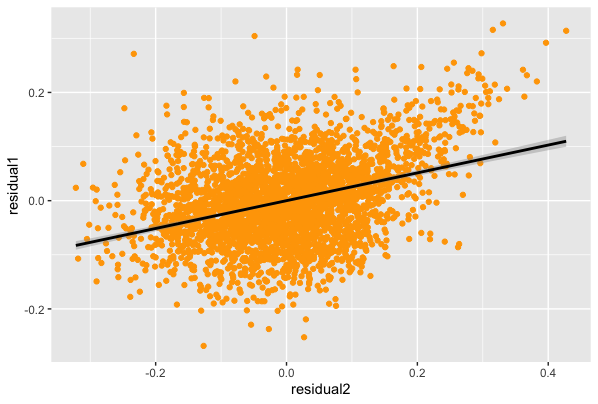
\includegraphics[width=.75\textwidth]{scatterplot4.png}
		\end{figure}
		
			\newpage	
		\noindent From the scatterplot for model4, We can see that there is a positive correlation between the two variables. The slope in the output of the previous question is positive, and the p value is less than 0.001, which verifies this as well.
		
		\vspace{1cm}
		
		\item Write the prediction equation.
		
						\begin{equation}
				\hat{\text{{residual1}}} =  0.2569 \times \text{{residual2}}
		\end{equation}
		
		\noindent The prediction equation of model4 means when the residual1 changes by one unit, the predicted voteshare changes by 0.2569 units. The multiple R-squared of this model is 0.130, indicating that the model can explain approximately 13.0\% of the variance in residual1. The  p-value of residual2 in the model is significant (p-value $<$ 0.05), indicating that residual2's prediction of residual1   is statistically significant.
		\end{enumerate}
		
		
		
		
		
	\end{enumerate}
	
	\newpage	

\section*{Question 5}
\noindent What if the incumbent's vote share is affected by both the president's popularity and the difference in spending between incumbent and challenger? 
	\begin{enumerate}
		\item Run a regression where the outcome variable is the incumbent's \texttt{voteshare} and the explanatory variables are \texttt{difflog} and \texttt{presvote}.	
		
		\noindent Input :
		\lstinputlisting[language=R, firstline=62, lastline=63]{PS3.R}  
		
		
		Output:
		\begin{verbatim}
			Call:
			lm(formula = voteshare ~ difflog + presvote, data = inc.sub)
			
			Residuals:    
			Min       1Q       Median     3Q        Max 
			-0.25928 -0.04737 -0.00121  0.04618  0.33126 
			
			Coefficients:            
			          Estimate  Std. Error   t value   Pr(>|t|)    
			(Intercept) 0.4486442  0.0063297   70.88   <2e-16 ***
			difflog     0.0355431  0.0009455   37.59   <2e-16 ***
			presvote   0.2568770  0.0117637   21.84   <2e-16 ***
			--Signif. codes:  0 ‘***’ 0.001 ‘**’ 0.01 ‘*’ 0.05 ‘.’ 0.1 ‘ ’ 1
			
			Residual standard error:  0.07339 on 3190 degrees of freedom
			Multiple R-squared:   0.4496,	Adjusted R-squared:      0.4493 
			F-statistic: 1303 on 2 and 3190 DF,  p-value: < 2.2e-16
			
		\end{verbatim}
		\normalsize
		
		\begin{table}[!htbp] \centering   \caption{}   \label{} \begin{tabular}{@{\extracolsep{5pt}}lc} \\[-1.8ex]\hline \hline \\[-1.8ex]  & \multicolumn{1}{c}{\textit{Dependent variable:}} \\ \cline{2-2} \\[-1.8ex] & voteshare \\ \hline \\[-1.8ex]  difflog & 0.036$^{***}$ \\   & (0.001) \\   & \\  presvote & 0.257$^{***}$ \\   & (0.012) \\   & \\  Constant & 0.449$^{***}$ \\   & (0.006) \\   & \\ \hline \\[-1.8ex] Observations & 3,193 \\ R$^{2}$ & 0.450 \\ Adjusted R$^{2}$ & 0.449 \\ Residual Std. Error & 0.073 (df = 3190) \\ F Statistic & 1,302.947$^{***}$ (df = 2; 3190) \\ \hline \hline \\[-1.8ex] \textit{Note:}  & \multicolumn{1}{r}{$^{*}$p$<$0.1; $^{**}$p$<$0.05; $^{***}$p$<$0.01} \\ \end{tabular} \end{table} 
		
		
		\vspace{7cm}
		\item Write the prediction equation.
		
			\begin{equation}
			\hat{\text{{voteshare}}} =  0.4486 + 0.0355\times\text{{difflog}} + 0.2569 \times \text{{presvote}}
		\end{equation}
		
		 	\noindent This regression equation provides a model for predicting vote share based on the values of the variables difflog and presvote. 0.4486 is the intercept term, indicating the expected vote share when both difflog and presvote are zero.  0.0355 is the coefficient for the variable difflog. For a one-unit increase in difflog, holding other variables constant, the predicted vote share is expected to increase by 0.0355.  0.2569 is the coefficient for the variable presvote. For a one-unit increase in presvote, under control of the remaining variables in the model, the predicted vote share is expected to increase by 0.2569.
		
		
		
			\vspace{5cm}
		\item What is it in this output that is identical to the output in Question 4? Why do you think this is the case?
		
		\noindent The  coefficient  of presvote  variable 0.2569 in the model5 is identical to the coefficient of the independent variable residual2 (0.2569) in the model 4. I will explain why the coefficients are the same with the help of the Venn diagram below.
		
		\vspace{1cm}
					\begin{figure}[h!]\centering
			\caption{\footnotesize Boxplot of $Y$ by $Region$.}\vspace{-1cm}
			\label{fig:plot_3c}
			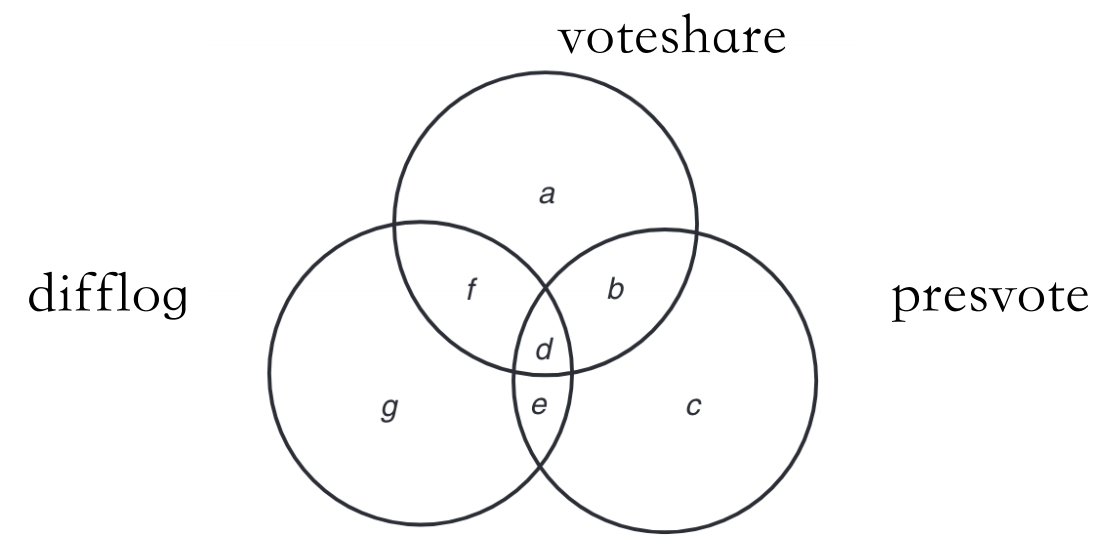
\includegraphics[width=.75\textwidth]{Venn Diagram.jpg}
		\end{figure}
		
		\vspace{1cm}
		
		\noindent In model1( difflog -> voteshare ), this binary regression equation only takes the effect of difflog variable into account. While In this venn figure, the relationship between difflog and voteshare - the area d+f - is affected by the presence of presvote. Therefore, the residual of model1 (residual1 as the dependent varable of model4) can be regarded as the consequence of omitted variable. In other words, residual1 represents the portion of the variation in voteshare that difflog cannot explain.  Presvote does contribute to explaining a portion of voteshare but be omitted in fact.
		
		In model2( difflog -> presvote), follow the same logic, the d portion of the variation in presvote is shared by both difflog and voteshare, so the residual of the binary regression equation ( denoted as residual2 in the model4) stands for the portion
		of the variation in presvote  unaccounted by difflog. 
		
		Back to model 4 (residual2 -> residual1), model 4 shows how the changes in presovte that difflog cannot explain affect the changes in voteshare that difflog cannot explain. In other words, except for the part contributed by difflog, the relationship between the remaining variables in the d area. And that is how, in the multiple regression model5, the parameter for presvote ,which represents the effects of presvote on voteshare, controls for the effects of difflog.  So the parameter 0.2569 in both equations is the same.
		
		
	\end{enumerate} 
	

\end{document}
